\documentclass[journal]{IEEEtran}

%\usepackage{ifpdf}
\usepackage{cite}
\usepackage{graphicx}
%\usepackage[cmex10]{amsmath}
%\usepackage{algorithmic}
%\usepackage{array}
\usepackage[caption=false,font=footnotesize]{subfig}
%\usepackage{fixltx2e}
%\usepackage{stfloats}
%\usepackage{dblfloatfix}
\usepackage{url}
\hyphenation{op-tical net-works semi-conduc-tor}

\begin{document}
\title{Hypercolumn-array Based Image Representation and 
Its Application to Shape-based Object Detection}
\author{Hui~Wei\thanks{Hui~Wei is with the School of Computer Science, 
Laboratory of Cognitive Modeling and Algorithms, 
Brain Science Research Center, Fudan University, Shanghai, China. 
Corresponding author's email: weihui@fudan.edu.cn.},
Zheng~Dong\thanks{Zheng~Dong and Qiang~Li are with the School of Computer Science, 
Laboratory of Cognitive Modeling and Algorithms, 
Fudan University, Shanghai, China.},
and~Qiang~Li}

% The paper headers
%\markboth{Journal of \LaTeX\ Class Files,~Vol.~13, No.~9, September~2014}%
%{Shell \MakeLowercase{\textit{et al.}}: Bare Demo of IEEEtran.cls for Journals}
%\IEEEpubid{0000--0000/00\$00.00~\copyright~2014 IEEE}
% Remember, if you use this you must call \IEEEpubidadjcol in the second
% column for its text to clear the IEEEpubid mark.

% make the title area
\maketitle

\begin{abstract}
Machine learning is perhaps the most popular strategy currently employed in object recognition. 
The strategy typically uses a high-dimensional vector to describe an image, 
and applies some classification algorithm to isolate positive areas apart from negative areas. 
While the advantage of this strategy is its architectural simplicity, 
it simultaneously suffers from computational complexity, fragile representation, 
unguaranteed generalization, black arts in optimization, and so on. 
In comparison with low-order features, such as color or gradient, contour is more stable and persistent; 
therefore, shape-based methods take account of a greater number of essential aspects for object recognition. 
Biological and psychological evidence increasingly reveals that geometrical and topological features are the keys to object recognition. 
Although these types of high-level features are not easily obtained, 
their discriminating abilities greatly improve the efficiency of perception. 
Attracted by the excellent performance of neural visual systems for shape processing, 
we simulate the mechanism of hypercolumns in the V1 cortex of mammals that selectively responds to bar stimuli, 
and design an orderly-arranged array to extract and represent all possible linear or near-linear stimuli in an image. 
Each unit of this array can cover all orientation stimuli occurring over a certain small area. 
These effective units together produce a type of low-dimensional vector to describe shape. 
Based on the neighborhood of units in the array, 
we construct a graph whose node represents a short line segment with a certain position and slope. 
Therefore, any segment of contour, i.e., a curve, in an edge image might be a route in that graph. 
The most significant thing here is that a graph converts an image, comprised of typically unstructured raw data, 
into structured and semantic-enriched data. 
We search along the routes in that graph and compare them with a shape template for object detection. 
Organizing segments of contour into a graph greatly upgrades the level of image representation, 
remarkably reduces the load of combinations, significantly improves the efficiency of object searching, 
and facilitates the intervening of high-level knowledge. 
This work provides a systematic infrastructure for shape-based models.
\end{abstract}

% Note that keywords are not normally used for peerreview papers.
\begin{IEEEkeywords}
orientation column, shape representation, object recognition, primary visual cortex.
\end{IEEEkeywords}

\IEEEpeerreviewmaketitle

\section{Introduction}

% needed in second column of first page if using \IEEEpubid
%\IEEEpubidadjcol

\IEEEPARstart{D}{etecting} 
an object within a complex background is still one of the major challenges of pattern recognition and computer vision. 
The difficulty lies in the conditions of image capture,
where images are captured under different illumination conditions, 
from different distances, and, sometimes, with overlapping objects.
These variations make an object's appearance, either in size, in posture, or in color, endless changing. 
While machine learning is arguably the most popular strategy currently employed in object recognition, 
the uncertainties associated with an ever changing environment and limited training create numerous difficulties for machine learning methods to achieve efficient object recognition. 
As such, obtaining an efficient, stable, and convenient method of representing features becomes the key requirement of object recognition in the real-world. 
The most stable characteristic of an object is its contour. 
The shapes or contours of most rigid objects tend to remain invariant regardless of a changing environment. 
Therefore, an object's shape or contour represents the most promising feature for efficient object recognition.


The primary visual cortex, which is also known as V1, locates in the striate cortex of mammals.
It is the best-studied visual area in the brain.
In this paper, we simulate the neural mechanism of V1 because this area contains many orderly-arranged hypercolumns that represent the orientation information of a visual stimulus.
This biological infrastructure provides a feasible entity to record object contours. 
We therefore design and train a self-organizing map (SOM) to extract the line information of an image. 
Under this approach, any line, regardless of its position, length, or slope, 
will activate one or more orientation-sensitive neurons, 
so an edge-image will be re-described by a set of active neurons. 
Based on this line-representing platform, 
we propose a contour-matching algorithm that uses geometrical characteristics to recognize objects. 
This provides good performance in environment adaptation and better generalization.

The remainder of this paper has been organized as follows. 
Section 2 reviews some related studies in shape-based object recognition and visual neurobiological mechanism simulation. 
The advantages and disadvantages of the main features of each study are briefly discussed. 
Section 3 presents the training process involving orientation columns, 
and how an image is represented by an array of artificial orientation columns. 
Section 4 describes how an edge image is converted into an undirected graph, 
and how route searching is conducted for this graph. 
Section 5 presents the method of similarity matching between routes and templates, 
and how this method is applied to the recognition of objects in real images. 
Experimental results are presented in Section 6, which is divided into two parts. 
Part one analyzes the capability for image representation and reduction provided by the proposed array of artificial orientation columns. 
Part two presents the recognition results obtained for some real image datasets. 
The final section presents conclusions and future expectations.

\section{Related Work}

Here, we divide the discussion of related work into two components. 
One component concerns the modeling of the V1 area, 
whereas the other component is concerned with shape- or contour-based object recognition methods. 

\subsection{V1 simulation research}

A number of approaches to the computational modeling of the neural mechanism of the V1 area of mammals have been proposed. 
The differences between these approaches lie in their points of focus, 
where some approaches focus on pathway, some on mechanism, and some on computation. 
Some studies have concentrated on the visual neural pathway 
\cite{bickle1999,shariati2012,nakagama2004,harvey2008}. 
For example, Bickle et al. \cite{bickle1999} proposed an artificial neural network with interactive activation and competition (IAC) mechanism by reference to the lateral geniculate nucleus (LGN), 
which is the direct pathway from the primary visual cortex to the thalamus, 
to implement several functions of the visual cortex. 
Shariati et al. \cite{shariati2012} simulated the entire neural pathway from a photoreceptor in the retina to the second sub-layer of the primary visual cortex. 
Some studies have concentrated on visual neurocomputing problems 
\cite{curuklu2002,wang2011,li2005,mihalas2011,ramirez2013}. 
For example, Curuklu \cite{curuklu2002} proposed a Bayesian confidence propagation neural network (BCPNN) to simulate a hypercolumn, which is the functional unit of the visual cortex. 
Wang et al. \cite{wang2011} used sparse coding and a back-propagation (BP) neural network to model the primary visual cortex. 
Finally, a number of studies have concentrated on the functional roles of variant neurons in the visual system \cite{okamoto2004,willmore2012,bednar2012,law2011,giacomantonio2010,zhao2010,yan2012,piech2013,song2013}. 
Okamoto \cite{okamoto2004} designed a honeycomb-like model based on a mechanism of short-range horizontal connections to explain the topological characteristics of the V1 area. 
Willmore \cite{willmore2012} successfully simulated the visual cortex based on Hebbian and anti-Hebbian rules. 
Bednar et al. \cite{bednar2012,law2011} implemented a gain-controlled, adaptive, 
and lateral-connected model that specialized the function of every neuron in the pathway, 
and simulated the primary visual cortex more completely. 
The above studies were able to realize some neural circuits and partial functions of the V1 area.
However, they did not sufficiently account for real image representation, 
which is the ultimate and most important function of the V1 area. 
In fact, all subsequent processing, such as object recognition and scene understanding, 
begins in the V1 area. 
Above all, these studies lacked the crucial consideration of how the V1's output meets the demands of subsequent recognition tasks. 
This constitutes one of the main goals of the present study.

\subsection{Shape- or contour-based object recognition}

Shape- or contour-based object recognition research has a long history. 
In the early stage, chamfer matching \cite{borgefors1988,shotton2005,thayananthan2003,opelt2006} 
was a frequently-used method that converted an original image into a depth image, 
and searched for the point with the best match. 
This method demonstrated a certain adaptability. 
As an additional aid, an image pyramid was designed to achieve scale invariance \cite{borgefors1988}. 
However, this method usually exhibits high time complexity and has a low tolerance to background interference. 
To address this problem, several new variants of the chamfer matching method have been proposed in recent years. 
For example, Shotton \cite{shotton2005} designed an oriented chamfer matching model, 
Thayananthan \cite{thayananthan2003} combined this method with a shape context descriptor, 
and Opelt \cite{thayananthan2003} added AdaBoost. 
These variants were observed to improve the efficiency and recognition rate.

Another type of shape-based method is mainly based on contour segment matching between templates and real images. 
This type of method firstly converts an image into edges, 
and then fits curves or line segments to the edge pixels. 
Subsequently, the set of curves or line segments are represented with some geometrical feature descriptors. Finally, the similarity between the set of segments and shape templates are obtained. 
Once matching pairs between line segments and the template are established, 
some guesses can be made to estimate the possible positions for the target object, 
and then verify these possible positions one-by-one. 
This type of method can be further divided into two categories. 
One is the dominant-set method and the other is the partial-match method. 
Pavan \cite{pavan2007} proposed the dominant-set method for finding the principle corresponding components in two sets. 
Yang \cite{yang2012} used this method to form a scale invariant global shape similarity estimation to match between template contour parts and image edge fragments. 
Partial-match methods \cite{ma2011,riemenschneider2010,liu2010} are similar to dominant-set methods. 
Ma \cite{ma2011} obtained a similarity matrix based on the angles of edges in a contour and maximized the similarity between classes through Liu's cluster algorithm \cite{liu2010}. 
Objects were then recognized by seeking the largest community. 
Differing from the work of Ma \cite{ma2011}, 
in the stage of evaluation, Riemenschneider \cite{riemenschneider2010} estimated the object position using the pyramid matching kernel (PMK) algorithm after conducting contour segment matching. 
Methods proposed in \cite{zhu2008,srinivasan2010} introduced a shape context descriptor. 
Zhu \cite{zhu2008} used linear programming to find a one-to-one mapping between the image and the template. 
Srinivasan \cite{srinivasan2010} developed this method further by introducing a bottom-up process to optimize many-to-one mapping results. 
In general all these methods exhibit high time complexity subject to exhaustive comparison between real-world images and templates.

Other shape-based recognition methods have been proposed, 
such as the constellation model \cite{fergus2004} and spectral model \cite{leordeanu2007}.
These methods use the relative location of points in a contour, 
where the established spatial relationships are regarded as constraints. 
The spatial relationships of an edge point to its surroundings are calculated in order to 
determine whether the surrounding pixels belong to the target object or to the background. 
A sparse representation is thus derived from these spatial relationships, 
and a probabilistic inference is used to estimate the position of a target object. 
The main disadvantage of this type of method is that the recognition result can be greatly affected 
when the foreground and the background are mixed or objects overlap. 
Leordeanu \cite{leordeanu2007} proposed a spectral model to calculate the geometrical relationships of pairwise points, 
and to analyze where pairwise points were densely located in a contour. 
The drawback of this model is that it requires a great many training samples.

In addition, some shape-based recognition methods are a mixture of several existing approaches. 
Fergus \cite{fergus2004} counted the occurrences of foreground features, 
and consulted with contour matching to obtain the probabilities of foreground to background, 
and, finally, to estimate the position of a target object. 
Gupta \cite{gupta2009} designed a contour descriptor by reference to the concept of torsion in physics. 
This descriptor performs well for changing scales. 
However, the method performs poorly when the contour is somewhat missing because it is concerned with global contours. 
Schlecht \cite{schlecht2011} described the marked features of an object by a codebook of angles, 
and combined Hough voting for object detection. 
Ferrari \cite{ferrari2006} proposed gradual contour searching to recognize objects in a real-world image.

In general, shape-based object recognition methods are not covered by the mainstream technology. 
The reasons for this are as follows. 
(a) This type of method always requires good preprocessing to reduce noise or to obtain some basic geometrical units such as line segments; however the preprocessing results are affected by numerous factors. 
(b) A target object’s background, position, size, and posture are changing constantly, 
which is a substantial challenge for template matching. 
(c) Template matching is essentially a combinational optimization problem that requires searching for a globally optimum solution, 
which is a severe challenge for any searching algorithm. 
(d) The template matching method involves many process steps such as template acquisition, 
template formal representation, search-friendly image re-organization and re-representation after preprocessing, 
definition of geometrical features, searching and combining geometrical features, 
definition of geometrical constraints, and generating and verifying assumptions. 
All these requirements increase the complexity of a complete shape-based system.

\section{Hypercolumn-array Based Image Representation}

\subsection{The structure of a hypercolumn-inspired array}

In \cite{wei2014,wei2014b,wei2000}, 
a multi-layer neural computational model that simulated hypercolumns in the primary visual cortex was proposed. 
The output layer of this model can be used to represent the orientation information of a contour image.

\begin{figure}[!t]
\centering
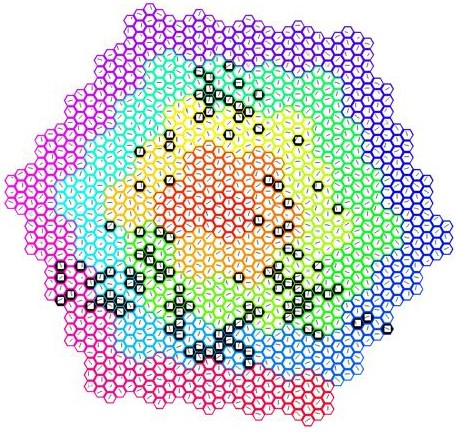
\includegraphics[width=0.85\linewidth]{images/fig1.jpg}
\caption{The structure of a hypercolumn-array, which is used for contour representation. 
Each small hexagon represents an orientation chip that corresponds to a simple cell. 
Each simple cell in the V1 area is sensitive to a bar of light with a particular orientation (slope). 
We evenly divide the overall orientation interval from 0 to $\pi$ into nineteen sub-intervals. 
Nineteen orientation chips, each of which responds to one, and only one, sub-interval, 
are combined as a hypercolumn, and nineteen small hexagons happen to form a large hexagon. 
All the chips in the same hypercolumn share the same receptive field.}
\label{fig:1}
\end{figure}

As shown in \figurename~\ref{fig:1},
this layer is comprised of a number of large, hexagonal hypercolumns, 
and two of these in the upper-right corner of the figure are marked by two black frames. 
Each hypercolumn consists of nineteen orientation chips (small hexagons). 
Each chip can selectively respond to an orientation-specific segment of contour existing in its receptive field. 
\figurename~\ref{fig:2} shows the scope and the distribution of the receptive fields of several neighboring hypercolumns, and how they share these receptive fields. 
All nineteen chips in a single column can completely cover the range of slope from 0 to $\pi$. 
All these columns assemble into an array, 
which plays the roles of extraction and representation of the orientation features of contour in an image. 

\begin{figure}[!t]
\centering
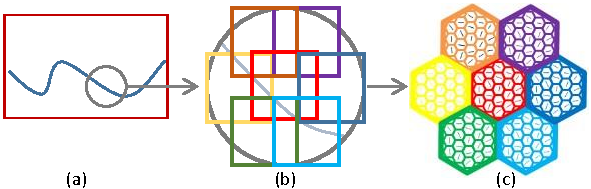
\includegraphics[width=\linewidth]{images/fig2.pdf}
\caption{Seven neighboring hypercolumns and their receptive fields in a visual field. 
(a) A segment of contour in a visual field. 
(b) The purple rounded region is covered by seven square receptive fields, 
and they overlap with each other to some extent. 
(c) Seven colored neighboring hypercolumns whose corresponding receptive fields with the same colors 
are shown in (b).}
\label{fig:2}
\end{figure}

\subsection{Representing images by a hypercolumn-inspired array}

One of the most important discoveries in neurobiology is that a hypercolumn in the primary cortex can respond to a series of stimuli with continuously changing orientations. 
As the discoverers, Hubel and Wiesel won the Nobel Prize in 1982. 
We were therefore inspired to use this mechanism to obtain and represent segments of contour in an image. 
After uploading an edge image to the aforementioned hypercolumn array, 
in a certain receptive field, 
some linearly-distributed pixels will activate a certain orientation chip of a hypercolumn. 
This indicates that we can represent all contour information in an image by a set of active units (i.e., orientation chips). In mathematics, each unit represents a line vector. Therefore, the output of a hypercolumn array is no longer a group of discrete, isolated, and pixel-wise points, 
but some preliminarily-integrated short line segments that contain a wealth of geometrical information such as position, length, and angle. 
Thus, the hypercolumn array not only upgrades the representation level of an edge image, 
but also reserves the original characteristic of pixel distribution in an edge image. 
\figurename~\ref{fig:3} to \figurename~\ref{fig:5} shows several examples of such representation.
A simple triangle, an onion shape, and a contour of a car were uploaded to the hypercolumn array,
which generated a set of activated orientation chips.
This is very similar to using sparse coding to represent an image.

\begin{figure}[!t]
\centering
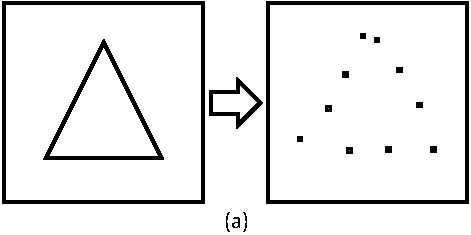
\includegraphics[width=0.55\linewidth]{images/fig3.pdf}
\caption{Some orientation chips (black points in (b)) are activated by a simple triangle in (a), 
where, in (b), the topological feature of the triangle is preserved by the set of active orientation chips.}
\label{fig:3}
\end{figure}

\begin{figure}[!t]
\centering
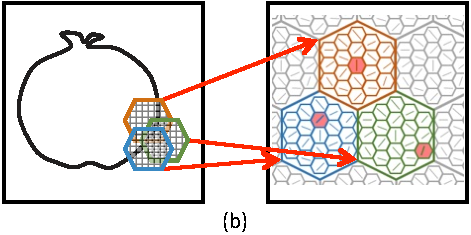
\includegraphics[width=0.55\linewidth]{images/fig4.pdf}
\caption{The partial contour at the bottom-right of an onion (in (a)) from the MPEG7 dataset 
passes through three neighboring and overlapping receptive fields, 
which activates three orientation chips in the three hypercolumns respectively (in (b)), 
and these chips correctly reflect the geometrical information in this contour segment.}
\label{fig:4}
\end{figure}

\begin{figure}[!t]
\centering
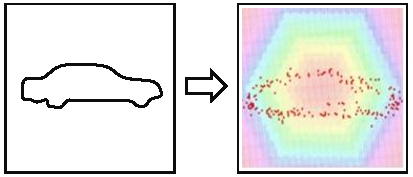
\includegraphics[width=0.55\linewidth]{images/fig5.pdf}
\caption{A contour of a car is represented by an array with 452 hypercolumns. 
The extent to which the details of the car that are preserved increases 
with an increasing number of activated orientation chips.}
\label{fig:5}
\end{figure}

The foregoing examples indicate that an edge image can be easily represented with activated orientation chips in a hypercolumn array. 
Each activated chip represents a vector reflecting the position, length, and angle of a short line segment. 
In addition, the chip's activation level can also indicate the level of similarity between a real stimulus and the chip's built-in preference. 
This is equivalent to a comparison between an input and a template. 
For example, the stimulus in a receptive field might sometimes be a curve or a dotted line rather than a perfect straight line. 
Therefore, the output of hypercolumns is an approximation to the original edge image, 
as shown in \figurename~\ref{fig:6}. 
This approximation can reflect the distribution of pixels in a receptive field, which offers a certain degree of flexibility and error tolerance.

\begin{figure}[!t]
\centering
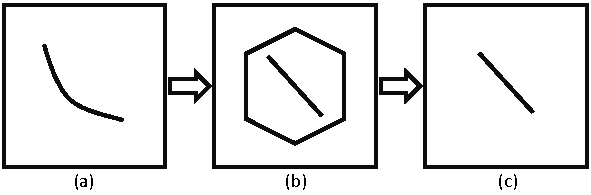
\includegraphics[width=0.6\linewidth]{images/fig6.pdf}
\caption{Orientation chips can approximately represent stimulus. 
(a) A real stimulus in a receptive field might be a small curve. 
(b) An orientation chip with the closest built-in orientation preference is activated. 
(c) The final output is an approximation of the original stimulus.}
\label{fig:6}
\end{figure}

\subsection{Image reconstruction from an activated array}

However, the scale of a hypercolumn-array, given as the number of hypercolumns in it, 
and the number of orientation chips in a hypercolumn, is limited. 
Thus, using a finite resource to represent infinite stimuli must inevitably result in approximation, 
and the degree of approximation must be evaluated after converting an original image to some activated orientation chips. 
To verify that the hypercolumn array can represent the original stimulus with sufficient fidelity, 
we rebuild an image by redrawing lines in the receptive fields of the activated orientation chips, 
and then compare the original image to the rebuilt one. 
As shown in \figurename~\ref{fig:7}, 
the contour information of an original image can be effectively recorded, 
and the rebuilt version is nearly identical to the original. 
Further experimental verification of the image reconstruction ability of a hypercolumn-array will be presented in Section 6.

\begin{figure}[!t]
\centering
\subfloat[Original image]{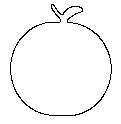
\includegraphics[width=0.25\linewidth]{images/fig7a.jpg}%
\label{fig:7a}}
\hfil
\subfloat[Rebuilt image]{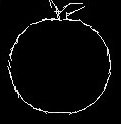
\includegraphics[width=0.25\linewidth]{images/fig7b.jpg}%
\label{fig:7b}}
\caption{The result of image reconstruction. (a) An original image from the MPEG7 dataset. (b) A rebuilt image based on the orientation chips activated by (a). Here, (a) and (b) are nearly identical.}
\label{fig:7}
\end{figure}

\section{Processing From A Hypercolumn Array To A Graph}

After the preprocessing of the hypercolumn array discussed in the previous section, 
an ordinary edge image has been converted to a group of active units, 
each of which represents a short line segment with a certain position, length, and slope, 
given as a quad vector: $x$-coordinate of the center point, 
$y$-coordinate of the center point, length, and slope. 
This representation by a group of units is more compact and information-rich. 
Compared with a complete contour, the line segment represented by an active unit is somewhat fine, 
and the information obtained from active units must be aggregated in some way to facilitate the subsequent recognition operation. 
The use of sets is a simple aggregation approach, 
but this approach is not sufficiently powerful to describe the topology of active units distributed in an array. 
The use of graphs is a more effective approach to describe the relations between adjacent or connected active units. 
Moreover, the layout characteristics of chips arranged in a hypercolumn as well as hypercolumns arranged in an array coincide with the functionality of graphs, 
where nodes and edges are two basic elements for constructing a graph. 
The analogy between a hypercolumn-array and a graph is quite a natural association. 
This suggests the application of graphs to describe the topological distribution of activated orientation chips.

\subsection{The generation of a graph}

We hope to represent a continuous contour by coordinating the information derived from multiple chips through the implementation of a graph. 
Therefore, the best manner of defining a graph for a hypercolumn-array is to set the chips as the nodes of the graph, 
and establish the edges between those nodes (i.e., chips) that might be successively joined together to represent a slightly longer line or curve. 
Because all 19 chips in a given hypercolumn share a completely coincident receptive field, 
and multiple lines are unlikely to exist concurrently in this fairly small area, 
these chips are usually not activated simultaneously.
Therefore, no edges can be established between these independent nodes. 
Only those chips with neighboring or partially overlapping receptive fields might be coordinated to represent a contour that passes through multiple receptive fields. 
Links are assigned between these possibly coordinated nodes that usually belong to separate but adjacent hypercolumns. 
The present description defines a basic graph of chip nodes, i.e., an orientation chip graph. 
Once an image has been uploaded, 
some nodes of this graph will be activated. 
Most importantly, the orientation chip graph provides a structural data form for subsequent geometrical or topological analysis, as illustrated in \figurename~\ref{fig:8}.

\begin{figure}[!t]
\centering
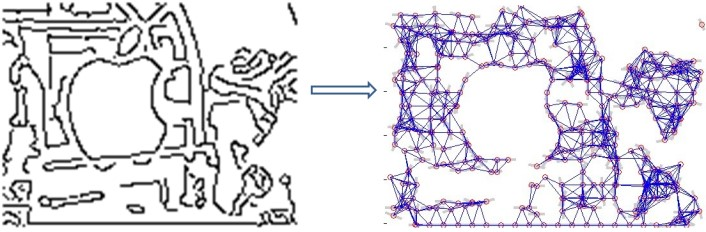
\includegraphics[width=0.85\linewidth]{images/fig8.jpg}
\caption{An edge image from the ETHZ dataset (at left) has activated some orientation chips. 
We can generate an undirected graph (at right), of which the nodes are these activated chips.}
\label{fig:8}
\end{figure}

\subsection{Graph searching and route-parsing}

The most significant value provided by the graph of chip nodes is 
(a) it effectively organizes raw image data, which is converted into an ordered structure, 
and (b) it facilitates the process of searching object contours. 
As indicated by the previous discussion, 
representing a continuous contour requires the coordination of multiple chips, 
which correspond to multiple connected nodes in our graph.
From the point of view of a graph, the sequence of these connected nodes forms a route.
\figurename~\ref{fig:9} shows an example of a route. 
The key to shape-based object recognition involves locating one or several such routes
that represent the contour or partial contour of the object to be discriminated.
Therefore, a route-searching algorithm is required.

\begin{figure}[!t]
\centering
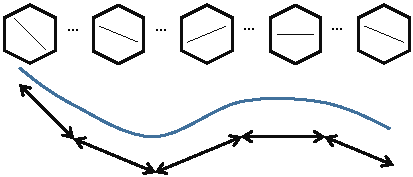
\includegraphics[width=0.65\linewidth]{images/fig9.pdf}
\caption{A segment of an object's contour might be a route of a chip graph. 
The top is a sequence of chips linked together by a route; 
the middle is the original stimulus that activated the above route; 
and the bottom is the approximate curve rebuilt from that route. }
\label{fig:9}
\end{figure}

Route-searching seeks to combine the neighboring nodes of a graph into routes that represent contour segments. 
However, some difficulties are encountered in this process because the contour of an object might suffer from interference with its background and be mixed with noise or be broken into several shorter segments.
As is shown in \figurename~\ref{fig:8}, 
the connectivity of a graph constructed from activated orientation chips can be high.
A randomly chosen long route might go through both an object and its background.
Ideally, a route should be either part of the object's contour or from the background,
and also it should convey enough information for us to determine whether it is part of the object's contour.
Therefore the searching process must be carefully guided to yield a reasonable result.
Natural contours tend to be smooth and continuous, which provides a good hint.
We assign weights to edges to measure the smoothness and continuity between chip nodes.
Given two adjacent nodes $u$ and $v$ in the chip graph,
the weight $w$ of the edge $(u,v)$ is defined as follows.
\begin{equation}
w(u,v) = e^{-\max\{dist(l(u), l(v)),\lambda\cdot|\alpha(u)-\alpha(v)|\}}.
\end{equation}
In this equation, $l(\cdot)$ is the short line segment represented by the corresponding orientation chip
and $\alpha(\cdot)$ is the orientation of that chip.
The function $dist(\cdot,\cdot)$ calculates the minimal distance between the endpoints of two line segments.
It measures the continuity between the two chips.
The difference of orientation is multiplied by a factor $\lambda$ to measure the smoothness.
In this paper, the orientation is measured in degree and $\lambda$ takes $0.15$.
The edge weights range from $0$ to $1$.
Larger weights indicate stronger collinearity between chip nodes.
\figurename~\ref{fig:10} illustrates weight setting in different cases.

\begin{figure}[!t]
\centering
\subfloat[$w=e^{-\max\{0,0\}}=1$]{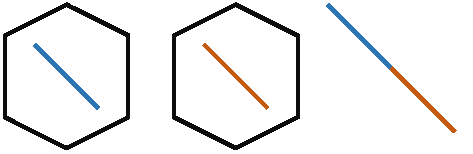
\includegraphics[width=0.45\linewidth]{images/fig10a.pdf}%
\label{fig:10a}}
\hfil
\subfloat[$w=e^{-\max\{0,15\lambda\}}=0.11$]{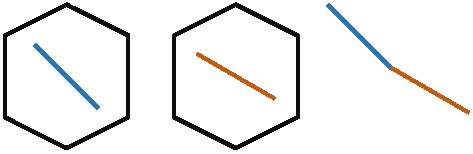
\includegraphics[width=0.45\linewidth]{images/fig10b.pdf}%
\label{fig:10b}}\\
\subfloat[$w=e^{-\max\{3,0\}}=0.05$]{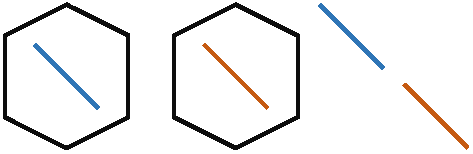
\includegraphics[width=0.45\linewidth]{images/fig10c.pdf}%
\label{fig:10c}}
\hfil
\subfloat[$w=e^{-\max\{0,35\lambda\}}=0.01$]{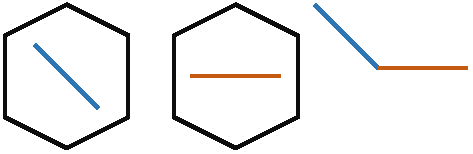
\includegraphics[width=0.45\linewidth]{images/fig10d.pdf}%
\label{fig:10d}}
\caption{Setting the edge weight between two orientation chips. 
A larger value indicates a tighter or more collinear connection.
(a) If two chips represent a longer line cooperatively, then the weight between them equals 1.
(b) If two chips represent a smooth curve, then the weight is relatively large.
(c) If two chips represent discontinuous short line segments, then the weight is small.
¨K: If two chips represent a sharp turn, then the weight is small.}
\label{fig:10}
\end{figure}


In the following algorithm, the route searching process is guided by edge weights.

  
% An example of a floating table. Note that, for IEEE style tables, the
% \caption command should come BEFORE the table and, given that table
% captions serve much like titles, are usually capitalized except for words
% such as a, an, and, as, at, but, by, for, in, nor, of, on, or, the, to
% and up, which are usually not capitalized unless they are the first or
% last word of the caption. Table text will default to \footnotesize as
% IEEE normally uses this smaller font for tables.
% The \label must come after \caption as always.
%
%\begin{table}[!t]
%% increase table row spacing, adjust to taste
%\renewcommand{\arraystretch}{1.3}
% if using array.sty, it might be a good idea to tweak the value of
% \extrarowheight as needed to properly center the text within the cells
%\caption{An Example of a Table}
%\label{table_example}
%\centering
%% Some packages, such as MDW tools, offer better commands for making tables
%% than the plain LaTeX2e tabular which is used here.
%\begin{tabular}{|c||c|}
%\hline
%One & Two\\
%\hline
%Three & Four\\
%\hline
%\end{tabular}
%\end{table}


% Note that the IEEE does not put floats in the very first column
% - or typically anywhere on the first page for that matter. Also,
% in-text middle ("here") positioning is typically not used, but it
% is allowed and encouraged for Computer Society conferences (but
% not Computer Society journals). Most IEEE journals/conferences use
% top floats exclusively. 
% Note that, LaTeX2e, unlike IEEE journals/conferences, places
% footnotes above bottom floats. This can be corrected via the
% \fnbelowfloat command of the stfloats package.




\section{Conclusion}
The conclusion goes here.





% if have a single appendix:
%\appendix[Proof of the Zonklar Equations]
% or
%\appendix  % for no appendix heading
% do not use \section anymore after \appendix, only \section*
% is possibly needed

% use appendices with more than one appendix
% then use \section to start each appendix
% you must declare a \section before using any
% \subsection or using \label (\appendices by itself
% starts a section numbered zero.)
%


\appendices
\section{Proof of the First Zonklar Equation}
Appendix one text goes here.

% you can choose not to have a title for an appendix
% if you want by leaving the argument blank
\section{}
Appendix two text goes here.


% use section* for acknowledgment
\section*{Acknowledgment}


The authors would like to thank...


% Can use something like this to put references on a page
% by themselves when using endfloat and the captionsoff option.
\ifCLASSOPTIONcaptionsoff
  \newpage
\fi



% trigger a \newpage just before the given reference
% number - used to balance the columns on the last page
% adjust value as needed - may need to be readjusted if
% the document is modified later
%\IEEEtriggeratref{8}
% The "triggered" command can be changed if desired:
%\IEEEtriggercmd{\enlargethispage{-5in}}

% references section

% can use a bibliography generated by BibTeX as a .bbl file
% BibTeX documentation can be easily obtained at:
% http://www.ctan.org/tex-archive/biblio/bibtex/contrib/doc/
% The IEEEtran BibTeX style support page is at:
% http://www.michaelshell.org/tex/ieeetran/bibtex/
\bibliographystyle{IEEEtran}
% argument is your BibTeX string definitions and bibliography database(s)
\bibliography{ref}
%
% <OR> manually copy in the resultant .bbl file
% set second argument of \begin to the number of references
% (used to reserve space for the reference number labels box)
%\begin{thebibliography}{1}
%
%\bibitem{IEEEhowto:kopka}
%H.~Kopka and P.~W. Daly, \emph{A Guide to \LaTeX}, 3rd~ed.\hskip 1em plus
%  0.5em minus 0.4em\relax Harlow, England: Addison-Wesley, 1999.
%
%\end{thebibliography}

% biography section
% 
% If you have an EPS/PDF photo (graphicx package needed) extra braces are
% needed around the contents of the optional argument to biography to prevent
% the LaTeX parser from getting confused when it sees the complicated
% \includegraphics command within an optional argument. (You could create
% your own custom macro containing the \includegraphics command to make things
% simpler here.)
%\begin{IEEEbiography}[{\includegraphics[width=1in,height=1.25in,clip,keepaspectratio]{mshell}}]{Michael Shell}
% or if you just want to reserve a space for a photo:

\begin{IEEEbiography}{Michael Shell}
Biography text here.
\end{IEEEbiography}

% if you will not have a photo at all:
\begin{IEEEbiographynophoto}{John Doe}
Biography text here.
\end{IEEEbiographynophoto}

% insert where needed to balance the two columns on the last page with
% biographies
%\newpage

\begin{IEEEbiographynophoto}{Jane Doe}
Biography text here.
\end{IEEEbiographynophoto}

% You can push biographies down or up by placing
% a \vfill before or after them. The appropriate
% use of \vfill depends on what kind of text is
% on the last page and whether or not the columns
% are being equalized.

%\vfill

% Can be used to pull up biographies so that the bottom of the last one
% is flush with the other column.
%\enlargethispage{-5in}



% that's all folks
\end{document}


